% This is samplepaper.tex, a sample chapter demonstrating the
% LLNCS macro package for Springer Computer Science proceedings;
% Version 2.20 of 2017/10/04
%
\documentclass[runningheads]{llncs}
%
\usepackage[utf8]{inputenc}
\usepackage{listings}
\usepackage{xcolor}
\usepackage{graphicx}
\usepackage{tabularx}
\usepackage{hyperref}

\graphicspath{ {./images/} }
\hypersetup{
    colorlinks=true,
    linkcolor=blue,
    filecolor=blue,
    citecolor=blue,
    urlcolor=blue,
    linktocpage=true
}
\setcounter{tocdepth}{2} %show more in the toc

\newcommand{\kw}[1]{\texttt{#1}}
\renewcommand{\contentsname}{table of content}
\usepackage{indentfirst}
\usepackage[english]{babel}

% If you use the hyperref package, please uncomment the following line
% to display URLs in blue roman font according to Springer's eBook style:
\renewcommand\UrlFont{\color{blue}\rmfamily}

%

\title{Infra-estrutura de Testes para Implementações de Referência do Standard ECMAScript}
\subtitle{}

%
\titlerunning{Live Metadata for Test262}
% If the paper title is too long for the running head, you can set
% an abbreviated paper title here
%
\author{Diogo Costa Reis\\ist187526\\
\email{diogo.costa.reis@tecnico.ulisboa.pt}}
%
\authorrunning{Diogo Costa Reis}
% First names are abbreviated in the running head.
% If there are more than two authors, 'et al.' is used.
%
\institute{Instituto Superior Técnico\\
Av. Rovisco Pais, 1\\
1049-001 Lisboa\\
Tel: +351 218 417 000\\
\email{mail@tecnico.ulisboa.pt}}
%


\begin{document}

% a solution to remove title and author from appearing in the table of contents: https://tex.stackexchange.com/a/318220
{\def\addcontentsline#1#2#3{}\maketitle}

%
\begin{abstract}
% TODO

\keywords{ECMAScript \and Specification Language \and Reference Interpreters \and Test262}
\end{abstract}


\newpage

\tableofcontents

\newpage

\section{Introduction}
\label{sec:Introduction}

\section{Goals}
\label{sec:Goals}

\section{Background}
\label{sec:Background}
This chapter provides an overview on the ECMAScript standard, the Test262 that are used to test the correct implementation of the ECMAScript standard, and finally an outline of the new metadata generated.

\subsection{ECMAScript}
\label{subsec:ECMAScript}
% overview da linguagem JS

% paragrafo - porque e' que javascript e' relevante (uma das linguagens mais usadas no momento)
JavaScript (JS) is a programming language mainly used in the development of client side web applications, also being one of the most popular programming languages. According to both GitHub and StakeOverflow statistics, JavaScript finished 2021 as second most active languages on GitHub\footnote{Second most utilized language based GitHub pull requests - https://madnight.github.io/githut/} as well as on StackOverflow.\footnote{Tendencies based on the Tags used - https://insights.stackoverflow.com/trends}




% Existem muitas implementacoes diferentes da linguagem: client-side (browsers), server-side (Node.js), embedded devices (Jerryscript) -> Estas implementacoes têm de estar de acordo no comportamento observavel -> é particularmente importante na Web -> senao temos sites que em ...
% -----------------------
% overview do standard -> descrita num standard
% Porque é muito importante que as várias implementacoes da linguagem coincidam -> o JavaScript está especificado num documento semi-formal que ...
% Falar sobre o standard
%   - o standard está como um interpretador de JavaScript em
%     pseudo-codigo - descreve detalhadamente os passos que
%    um interpretador de JS tem de executar ao avaliar qualquer
%    statement da linguagem
% Falar sobre o comité -  quem controla a evolucao do ECMAScript
ECMAScript standard\cite{ECMAScriptStandard} is the official document, written in the English language, in which the JavaScript language is defined. This document is in constant evolution, being updated by the ECMA Technical Committee 39 (TC39), which is responsible for maintaining the standard. The standard is currently in its twelfth version.
%
The standard specifies the \texttt{JavaScript} language, to ensure it's multiple compilers and interpreters implementions are coherent. Some of the \texttt{JavaScript} compilers are the ~\cite{Hop} and the JSC~\cite{JSC} compilers, the most popular interpreters are nodejs~\cite{nodejs} and spidermonkey~\cite{spidermonkey}. These are only four implementations amongst many others, which come along with the many use cases that \texttt{JavaScript} has.
%
\texttt{JavaScript} is used mostly used in the web context, both client-side within browsers and server-side, but also in embedded devices. Since \texttt{JavaScript} is used in so many scenarios and across so many different contexts, there is highly important that ECMAScript standard is defined in great detail to ensure consistency. Browsers, for example, need to run \texttt{JavaScript} implementations that coincide so that websites are correctly rendered. In order to achieve coherent implementations, the standard defines the types, values, objects, properties, syntax, and semantics of \texttt{JavaScript} that must be the same in every \texttt{JavaScript} compiler and interpreter, while allowing \texttt{JavaScript} implementations to define additional types, values, object, properties, and functions.




% Good, more detail if there is time
% Estrutura do standard
The \texttt{JavaScript} language can be divided into three major components, those being expressions and commands, built-in libraries, and finally internal functions.
%
\begin{itemize}
\item Expressions and commands describe the behavior of static constructions, detailing the semantics of the diverse expressions (e.g., assignment expressions, built-in operators, etc.), commands (e.g., loop commands, conditions command, etc.), and built-in types (Undefined, Null, Boolean, Number, String and Object).
%
\item The internal functions of the language are used to define the semantics for both expressions and commands, as well as the built-in libraries. Internal functions are not exposed beyond the internal context of the language. In other words, no JavaScript program uses internal functions directly.
%
\item Finally, built-in libraries encompass all the internal objects available when a JavaScript program is executed. Internal objects expose many functions implemented by the language itself, including functions to manipulate numbers, text, arrays, objects, amongst other things.
\end{itemize}


% MetaParagrafo tres tipos
The remaining subsection provides a description of the three types of artifact described in the standard.

% Expressions and statements
% Exemplo do standard  e explicacao (if)
\paragraph{Semantics of IF statement}
Figure \ref{fig:If-Else Statement} shows a snippet of the ECMAScript standard description of the \texttt{IF} command. In order to evaluate \texttt{IF} commands with the shape:

\begin{center}
\texttt{if (Expression) Statement1 else Statement2}
\end{center}

\noindent the language begins by evaluating the \texttt{Expression} storing the result in the variable \texttt{exprRef} (step 1). The previous step will be used as Boolean, therefore, the result of the previous step will be converted to a Boolean using the internat functions \texttt{ToBoolean} and \texttt{GetValue}, and having the result stored in the variable \texttt{exprValue} (step 2).A different \texttt{Statement} will be followed depending on \texttt{exprValue}. If \texttt{exprValue} has the value \texttt{true} the variable \texttt{stmtCompletion} will have the evaluation of the first \texttt{Statement} (step 3). Otherwise, the variable \texttt{stmtCompletion} will store the result of evaluating the second \texttt{Statement} (step 4). Finally, a \texttt{Completion} will be returned, if the \texttt{stmtCompletion} has non empty value then it will be returned, however, when the value is empty it will be replaced with undefined (step 5).

\begin{figure}[ht]
    \centering
    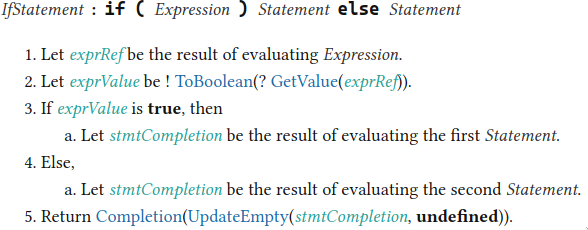
\includegraphics[width=0.8\textwidth]{images/if_statement.png}
    \caption{ECMAScript definition of an if-else statement}
    \label{fig:If-Else Statement}
\end{figure}

% arrays são objetos como os outros
% arrys tem propriedades especiais
% example of Array.pop
% Built-ins (Array.pop)
% printscreen do standard e explicacao
\paragraph{Semantics of the Pop function}
The Array built-in is an object as any other in JavaScript. The main difference is in its properties. Array Objects have a property \texttt{length} that contains the size of the array, as well as a property for each element of the array (from zero to \texttt{length} minus 1).

Figure \ref{fig:Array_pop_example} shows a simplified version of an array performing the pop function, where \texttt{(a)} and \texttt{(b)} are the before and after respectively.
Before preforming \texttt{pop} \texttt{(a)}, the array has three  properties \texttt{length}, \texttt{0}, and \texttt{1}. Property \texttt{length} represents the size of the array that has value \texttt{2}. While the properties \texttt{0} and \texttt{1} store the first (\texttt{banana}) and second (\texttt{kiwi}) elements of the array respectively.
After \texttt{pop} being preformed \texttt{(b)}, the last element is of the array is removed (highlighted in red at \texttt{(a)}). The \texttt{length} property highlighted in green is also updated since the size of the array changes to one.

% TODO change length with quotation marks
\begin{figure}[ht]
    \centering
    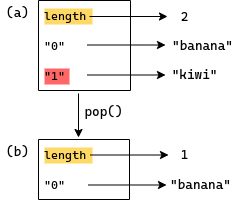
\includegraphics[width=0.4\textwidth]{images/array_pop_example.png}
    \caption{Example Array.pop}
    \label{fig:Array_pop_example}
\end{figure}
Figure \ref{fig:Array_pop} shows a snippet of the ECMAScript standard description of the pop function in the Array Built-in. To begin with, the array will be converted to and Object using the \texttt{ToObject} function, and stored in the \texttt{O} variable (step 1).
Afterwards, the array length of the previously calculated variable will be calculated with the \texttt{LengthOfArrayLike} internal function, and storing the result in the \texttt{len} variable (step 2).
At this point there are to ways to proceed depending on the value of \texttt{len}. If the value is zero, the Array is empty, then the property \texttt{length} of \texttt{O} is set to zero and \texttt{undefined} is returned (step 3).
Otherwise, when \texttt{len} is different from zero, meaning that the Array is not empty, the Array's last element will be removed (described in Figure \ref{fig:Array_pop_example}) and returned (step 4).
To begin with, the language will assert that \texttt{len} is positive (step 4.a).
Afterwards, the \texttt{newLen} variable will store the value of \texttt{len} decremented by 1 (step 4.b).
The variable \texttt{index} will store the variable calculated in the previous step represented as a String converted with the \texttt{toString} function (step 4.c).
Then, stores the value of the \texttt{O} variable at the property corresponding to \texttt{index} in the \texttt{element} variable using the \texttt{Get} function (step 4.d).
Subsequently, deletes the previously mentioned property of the \texttt{O} variable with the \texttt{DeletePropertyOrThrow} function (step 4.e).
In addition, sets the \texttt{length} property of the \texttt{O} variable  to the \texttt{newLen} using the \texttt{Set} function (step 4.f).
Finally, returning the value of the variable \texttt{element} (step 4.g).

\begin{figure}[ht]
    \centering
    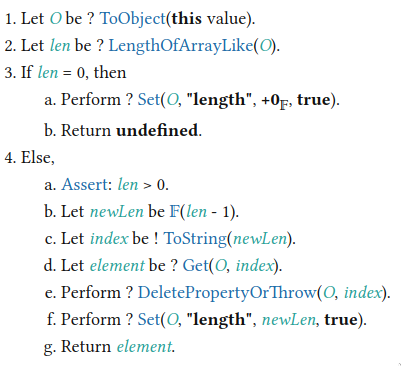
\includegraphics[width=0.6\textwidth]{images/array_pop.png}
    \caption{ECMAScript definition of Array.pop}
    \label{fig:Array_pop}
\end{figure}



% Internal Functions (LenghtOfArrayLike)
% printscreen do standard e explicacao
\paragraph*{LengthOfArrayLike internal function}
Figure \ref{fig:LengthOfArrayLike} shows a snippet of the ECMAScript standard description of the \texttt{LengthOfArrayLike} internal function, that evaluates the function:

\begin{center}
\texttt{LengthOfArrayLike (obj)}
\end{center}

\noindent The language starts by asserting that \texttt{obj} is an \texttt{Object} (step 1). Afterwards, gets the value of the property \texttt{length} from \texttt{obj} using the function \texttt{Get}. Then, converts the previously mentioned value to an Integer that represents the length with the \texttt{ToLength} function, and finally returns said Integer (step 2).

\begin{figure}[ht]
    \centering
    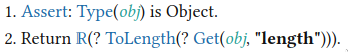
\includegraphics[width=0.5\textwidth]{images/length_array_like.png}
    \caption{ECMAScript definition of the LengthOfArrayLike}
    \label{fig:LengthOfArrayLike}
\end{figure}




\subsection{Test262}
\label{subsec:Test262}


% paragrafo - JS tem muitas particularidades que dificultam o desemvolvimento e testagem  -> É muito dificil desenvolver
% novas implemenentacoes da linguagem
% Existe uma bateria de testes que testa as implementacoes da
% linguagem contra o standard
% Esta bateria de testes é dificil de manter
% Porque? - muitos testes, muitas features, em geral ha retrocompatibilidade mas ha um pequeno numero de casos onde a retrocompatibilidade nao se verifica -> os testes de ser modificados
Implementing a \texttt{JavaScript} engine is particularly difficult since it involves dealing with the many corner cases that exist in the language. To test that corner cases are \colorbox{orange}{correctly dealt with there is \texttt{Test262}\cite{Test262}}, the ECMAScript standard test battery. Although, \texttt{Test262} is vital to the \texttt{JavaScript} engines, it is very hard to maintain due it's complexity (large quantity of tests and features).\texttt{Test262} complexity grows with changes to the standard since in most cases retrocompatibility is maintained except for a few select cases. 
%
% doesn't that imply wrongly that Test262 is comple???
%


% Implementacoes parciais da linguagem
% Na acadamia é normal desenvolverem-se implementacoes parciais da linguagem: não suportam a ultima versao, não suportam todos os objectos built-in, não suportam todas
% Pergunta: Quais é que são os testes apropriados?
% Normal: Respostas ad-hoc -> sem justificação rigorosa -> basicamente cada paper selecciona os testes que lhe da jeito
Due to ECMAScript standard being so extensive most implementations are only partial (namely implementations in academic context). Since the implementations are only partial, only tests for features that are implemented are relevant. Since selecting the relevant tests is not a trivial matter, each development team selects the appropiate tests. Each development selecting the tests raises the problem that there is not standard and precise way of picking the all the right tests.



%%
%% Formato dos testes
% frontmatter, code
% exemplo
Figure \ref{fig:Test262_example} shows a test from \texttt{Test262}. Every test of test262 has 3 parts: first is the copyright section represented with the comment \texttt{//} (lines 1 and 2), second is the \texttt{Frontmatter} section between \texttt{/*---} and \texttt{---*/} with some metadata about the test (lines 4 to 7), and finally is the \texttt{Body} section with the code of the test (lines 9 to 12). The copyright section has information about the owner and licence of the test. The \texttt{Frontmatter} section has the the test id (15.4.5-1) and a description of the test. Finally, the \texttt{Body}'s code tests the correct implementation of the standard.

\begin{figure}[ht]
    \centering
    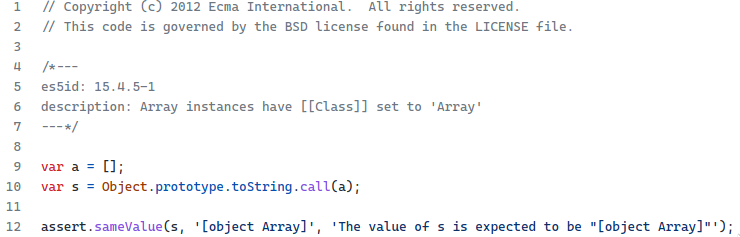
\includegraphics[width=1.2\textwidth]{images/test262_array_test.png}
    \caption{Test262 es5id: 15.4.5-1}
    \label{fig:Test262_example}
\end{figure}



%% metadados ja incluidos
%% referir outra vez o exemplo
% - metadados oficialmente incluídos nos testes
%   - que metadados é que os testes contém actualmente
The \texttt{Frontmatter} has keywords to hold metadata of the test. These keywords are associated with some type of metadata about the test. Bellow is the list of possible keywords and its meaning:

\begin{itemize}
\item \texttt{description} - contains a short description about what will be tested;
%
\item \texttt{esid} - contains the hash identifier of the ECMAScript portion associated with the feature that will be tested (the identifier references the most recent version of ECMAScript when the test is created);
%
\item \texttt{info} - contains a deeper explanation of the test behavior, frequently includes a direct citation of the standard;
%
\item \texttt{negative} - indicates that the test throws an error; associated to the keyword will be the type of error the test is supposed to throw (e.g. \texttt{TypeError}, \texttt{ReferenceError}) as well as the phase in which the error is expected to be thrown (e.g. \texttt{parse} vs \texttt{resolution} vs \texttt{runtime});
%
\item \texttt{includes} - contains the list of harness files that should be included in the execution of the tests;
%
\item \texttt{author} - contains the identification of the author of the test;
%
\item \texttt{flags} - contains a list of booleans for each property. The properties being: 1 \texttt{onlyStrict}, the test is only executed in strict mode; 2 noStrict, the test will only be executed in mode "sloppy"; 3 \texttt{module}, the test must be integrated as a \texttt{JavaScript} module; 4 \texttt{raw}, executes the test without any modification, which implies running as \texttt{noStrict}; 5 \texttt{async}, only for asyncronus tests; 6 \texttt{generated}, flag that identifies files created by a test; 7 \texttt{CanBlockIsFalse} and 8 \texttt{CanBlockIsTrue}, indicatethe value of the property \texttt{CanBlock} ; 9 \colorbox{orange}{\texttt{non-deterministic}}, idicates that the semantics used on the test are intentionally under-specified and therefore the test passing or failing should not be regarded as an indication of reliability or conformance;
%
% non-deterministic nao esta na tese do miguel trigo
%
%
\item \texttt{features} - containds a list of features that are used in the test;
%
\item \texttt{es5id} and \texttt{es6id} - indicates that the feature being tested belongs to ECMAScript 5 and 6 respectively and contains the hash identifier of the section of the standard it bellongs to; these keywords have been deprecated and substituted by esid;
\end{itemize}

%% metadados que achamos relevantes e nao estao incluidos
%% ...
The example in \ref{fig:Test262_example} has 2 keywords, description and the deprecated es5id. Besides the obvious upgrade from \texttt{es5id} to \texttt{esid} it would be usefull to have \texttt{includes} with the harness files needed to execute the test. The harness information is very usefull since it makes easly available what part of the harness is needed to run that test, opening the door for loading only part of the harness instead of the whole harness which is the current approach.



% - quais são os metadados que nós achamos serem relevantes e que estão em falta
In order to have a more complete \texttt{Frontmatter} we suggest adding the following information:

\begin{itemize}
    \item \texttt{static construct} - list of static constructions used in the test
    \item \texttt{version} - the ECMAScript version of the standard after which the test belongs to
    \item \texttt{built-ins} - list of all the built-ins used in the test
\end{itemize}

This metadata provides helpfull information to solve the problem mentioned before of selecting the relevant tests for partial implementations. 

\subsection{An Infrastructure for testing reference implementations of the ECMAScript standard}
\label{subsec:An Infrastructure for testing reference implementations of the ECMAScript standard}

%% Metodologia
% - metadados da Test262 -> estruturados

% - quais são os novos metadados incluídos

% - sumário das abordagens utilizadas para os calcular

% - shortcomings...

\section{Related Work}
\label{sec:Related Work}


\section{Design and Methodology}
\label{sec:Design and Methodology}

\section{Evaluation and Planning}
\label{sec:Evaluation and Planning}


\section{Conclusion}
\label{sec:Conclusion}


%
% the environments 'definition', 'lemma', 'proposition', 'corollary',
% 'remark', and 'example' are defined in the LLNCS documentclass as well.
%

%
% ---- Bibliography ----
%
% BibTeX users should specify bibliography style 'splncs04'.
% References will then be sorted and formatted in the correct style.
%
% \bibliographystyle{splncs04}
% \bibliography{mybibliography}
%
\bibliographystyle{splncs04}
\bibliography{references}

\end{document}
